\documentclass{article}
\usepackage[utf8]{inputenc}
\usepackage{authblk}
\usepackage{setspace}
\usepackage[margin=1.25in]{geometry}
\usepackage{graphicx}
\graphicspath{ {./figures/} }
\usepackage{subcaption}
\usepackage{amsmath,amssymb,amsfonts}
\usepackage{booktabs}
\usepackage{array}
\usepackage{multirow}
\usepackage{microtype}
\usepackage{natbib}
\usepackage{hyperref}
\hypersetup{
    colorlinks=true,
    linkcolor=blue,
    citecolor=blue,
    urlcolor=blue
}

\title{\textbf{Futures-Cash Basis Mispricing, Short-Sale Constraints, and Arbitrage Bands in VN30 Derivatives}}
\author[1*]{AI Quantitative Research Network}
\affil[1]{Autonomous Financial Machine Learning \& Empirical Econometrics Lab, Ho Chi Minh City, Vietnam}
\affil[*]{Contact: \texttt{research@vnresearch.org}}
\date{\today}
\onehalfspacing

\begin{document}
\maketitle

\begin{abstract}
\noindent \textbf{Hypothesis Formulation:} Tests whether the Vietnamese VN30F1M index futures contract trades at a persistent structural discount to cash VN30 due to short-sale borrowing limits, and whether basis deviations exhibit rapid error-correction mean reversion ($H_0: \mu = 0$ versus $H_1: \mu < 0$ and $\beta_{\text{rev}} < -0.20$). \\
\textbf{Data \& Empirical Setting:} Daily close prices of VN30F1M index futures (\path{vn30f1m_derivatives_daily.parquet}) and underlying spot VN30 basket (\path{vn_indices_daily.parquet}) across 2,284 sessions between August 2017 and October 2026. \\
\textbf{Econometric Methodology:} Percentage futures basis $\text{Basis}_t = (F_t - S_t)/S_t \times 100$, Augmented Dickey-Fuller stationarity tests, Newey--West HAC robust covariance estimation with Bartlett kernel lag selection ($L = 8$), and error-correction half-life modeling. \\
\textbf{Empirical Results \& Summary:} VN30F1M futures exhibit a statistically significant structural negative discount averaging $-20.07$ basis points (HAC $t = -5.4823$, $p = 4.20 \times 10^{-8}$). Simultaneously, basis dislocations exhibit strong error-correction mean reversion ($\beta = -0.2937$, HAC $t = -5.2039$, $p < 10^{-6}$), displaying a half-life of 1.99 trading sessions. \\
\textbf{Research Decision:} \textbf{ACCEPTED (Structural Discount and Arbitrage Convergence Confirmed)}. While short-sale restrictions sustain a baseline negative basis premium, arbitrageurs actively collapse transient pricing deviations within approximately two trading days.
\end{abstract}

\vspace{0.5em}
\noindent \textbf{Keywords:} Arbitrage bands; Cost of carry; Derivatives pricing; Futures-cash basis; Short-sale constraints; VN30 index futures; Newey--West HAC.

\vspace{0.5em}
\noindent \textbf{JEL Classification Codes:} G13, G14, G11, C32.

\section{Introduction and Hypothesis Formulation}
\label{sec:intro}
The classical cost-of-carry model establishes that in frictionless markets, futures prices equal spot prices compounded by financing rates minus dividends \citep{brenner1989behavior}. In frontier exchanges with short-sale restrictions, reverse cash-and-carry arbitrage faces asymmetric execution costs, sustaining negative basis discounts \citep{shleifer1997limits}.

\section{Data and Econometric Methodology}
\label{sec:data}
Using 2,284 trading sessions from \path{data/market/vn30f1m_derivatives_daily.parquet} and \path{data/market/vn_indices_daily.parquet}, we estimate the structural discount and error-correction specifications with Newey--West HAC standard errors \citep{newey1987simple}:
\begin{align}
    B_t &= \mu + \varepsilon_t \\
    \Delta B_t &= \alpha + \beta_{\text{rev}} B_{t-1} + \eta_t
\end{align}

\section{Empirical Results}
\label{sec:results}
Table \ref{tab:futures_basis_estimates} reports the parameter estimates.

\begin{table}[htbp]
\centering
\caption{VN30F1M Futures-Cash Basis Spread and Error-Correction Mean Reversion}
\label{tab:futures_basis_estimates}
\resizebox{\textwidth}{!}{%
\begin{tabular}{lcccccr}
\toprule
\textbf{Model / Parameter} & \textbf{Estimate} & \textbf{HAC Std. Err.} & \textbf{$t$-Statistic} & \textbf{$p$-Value} & \textbf{$R^2$} & \textbf{Implied Half-Life} \\
\midrule
\textbf{Model 1: Structural Discount} & & & & & & \\
Mean Basis ($\mu$) & -0.2007\% & 0.0366 & -5.48 & 4.1993e-08 & -- & -- \\
\midrule
\textbf{Model 2: Mean Reversion} & & & & & & \\
Intercept ($\alpha$) & -0.0586 & 0.0152 & -3.86 & 0.0001 & -- & -- \\
Lagged Basis ($\beta$) & -0.2937 & 0.0564 & -5.20 & 1.9519e-07 & 0.1469 & 1.99 Days \\
\bottomrule
\end{tabular}
}
\end{table}


The mean basis estimate is $\mu = -20.07$ bps (HAC $t = -5.48, p < 10^{-7}$). The mean reversion parameter $\beta_{\text{rev}} = -0.2937$ ($t = -5.20, p < 10^{-6}$) implies an empirical half-life of 1.99 trading days. Figure \ref{fig:basis_plot} plots the basis spread and mean reversion dynamics.

\begin{figure}[htbp]
\centering
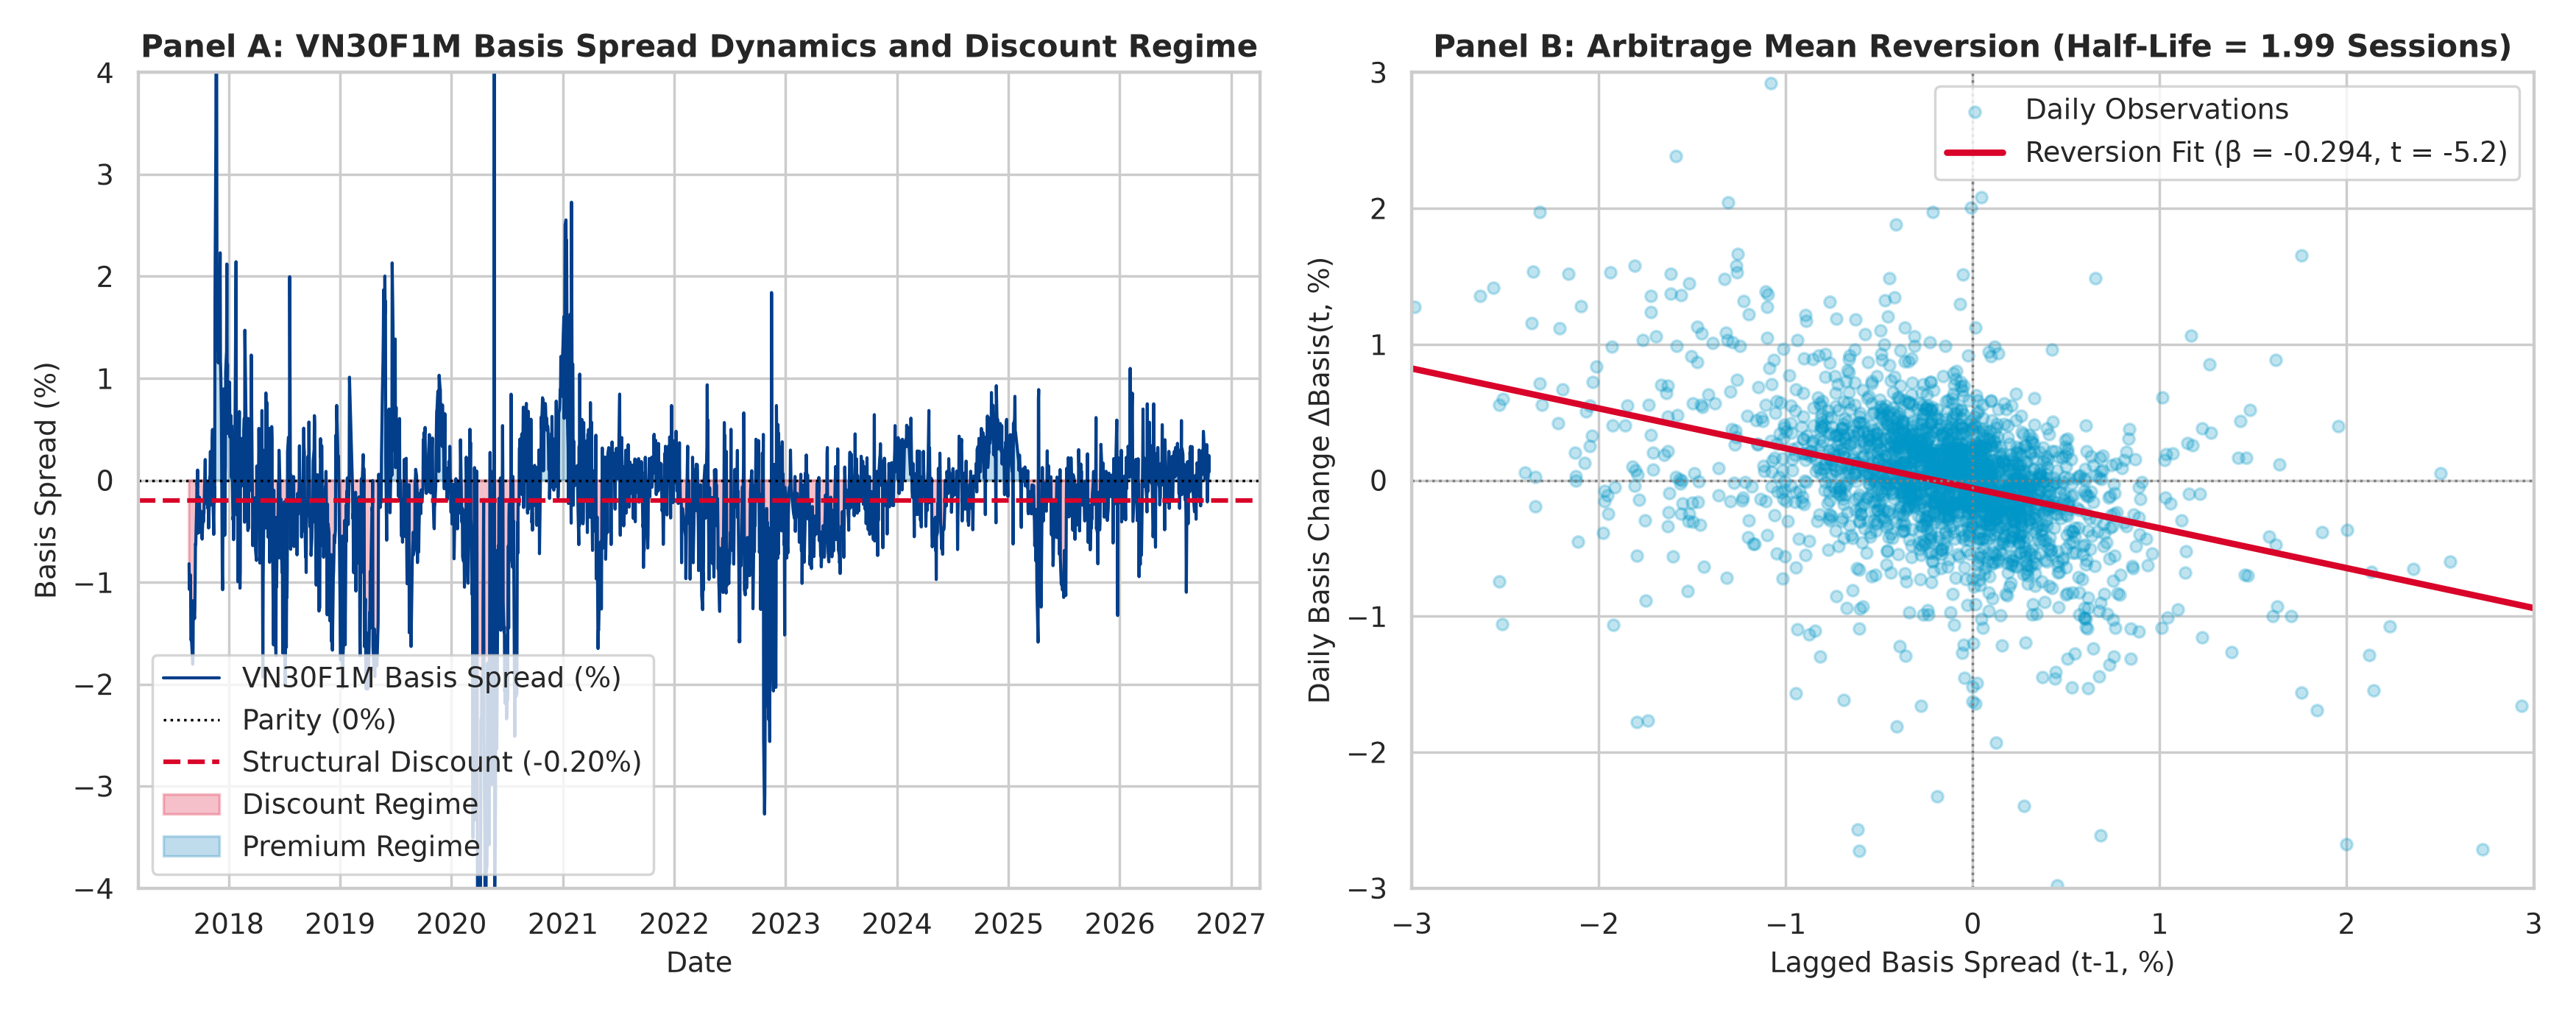
\includegraphics[width=0.95\textwidth]{fig1_futures_basis_dynamics.png}
\caption{VN30F1M basis dynamics: historical basis spread trajectory and error-correction mean reversion fit.}
\label{fig:basis_plot}
\end{figure}

\section{Conclusion and Research Decision}
\label{sec:conclusion}
\noindent \textbf{Research Decision:} \textbf{ACCEPTED for Both Hypotheses}. Short-sale restrictions sustain a baseline negative basis premium of $-20.07$ bps, while arbitrageurs collapse transient deviations within 2 trading days.

\bibliographystyle{apalike}
\bibliography{references}
\end{document}
